\documentclass[twocolumn]{layout/tudelft-aiaa}

%% Additional packages and commands
\renewcommand{\deg}{\si{\degree}\xspace}
\usepackage{parskip}
\usepackage{cleveref}
\usepackage{eurosym}
\usepackage{amsmath}
\usepackage{graphicx} 
\usepackage{hyperref}
%\usepackage{natbib}



%% Defining title, author and affiliation
\title{RL-MPC for Autonomous Greenhouse Control}
\author{Murray Harraway}
\affil{Delft Center for Systems and Control}

%%%%%%%%%%%%%%%%%%%%%%%%%%%%%
%%%%% Begin of document %%%%%
%%%%%%%%%%%%%%%%%%%%%%%%%%%%%

\begin{document}

\AlwaysPagewidth{

\maketitle

%% Abstract

\begin{abstract}
      The efficient operation of smart greenhouses is essential for enhancing crop yield while minimizing energy costs. This paper investigates a hybrid control strategy that integrates Reinforcement Learning (RL) and Model Predictive Control (MPC) to optimize economic benefits in autonomous greenhouses. While previous research has explored the use of RL and MPC individually, this study examines the effect of modifying MPC’s objective function with terminal constraints and a cost function informed by an independently trained RL agent. This approach leverages RL's ability to handle uncertainties and MPC’s online optimisation to improve overall control performance in both a deterministic and stochastic environment. Simulation results demonstrate that in a deterministic environment, RL-MPC outperforms both MPC and RL, particularly showing greater performance gains at lower prediction horizons. Additionally, the results indicate that RL trained in an uncertain environment can transfer its understanding of uncertainty into the RL-MPC framework. This integration allows RL-MPC to maintain superior performance in low uncertainty conditions while exhibiting greater robustness compared to MPC under higher uncertainties.
\end{abstract}

}

%% Nomenclature

\renewcommand{\nompreamble}{\emph{Use this section to provide a list of all symbols used in the report. Provide a concise description. For example:}} %

\printnomenclature[\nomequalsign]

\nomenclature{$A$}{amplitude of oscillation}
\nomenclature{$C_p$}{pressure coefficient}
\nomenclature{$C_x$}{force coefficient in the x direction}
\nomenclature{$C_y$}{force coefficient in the y direction}
\nomenclature{$c$}{chord}
\nomenclature{$dt$}{time step}
\nomenclature{$F_x$}{X component of the resultant pressure force acting on the vehicle}
\nomenclature{$F_y$}{Y component of the resultant pressure force acting on the vehicle}
\nomenclature{$f, g$}{generic functions}
\nomenclature{$h$}{height}
\nomenclature{$i$}{time index during navigation}

%% Main body

\chapter{Introduction}
\label{chapter:introduction, written in the present tense}

The world population is set to increase to a staggering 10 billion people in the year 2050 \cite{blazhevskaGrowingSlowerPace2019}, increasing food demand substantially. Currently, 800 million people are chronically hungry, with 2 billion people suffering from micronutrient deficiencies \cite{faoFutureFoodAgriculture2017}.The situation is compounded by the anticipated rise in food demand, which is expected to increase from 30\% to 62\% between the years 2010 and 2050, resulting in 30\% of the population being at risk of hunger \cite{vandijkMetaanalysisProjectedGlobal2021}. As such, there is a pressing need to enhance food production by at least 70\% \cite{nishatGreenDealGreenhouse2020}. Although large investments have been made to increase food productivity, food losses, waste, and climate change continue to serve as significant constraints \cite{faoFutureFoodAgriculture2017}. To meet these food demands, agriculture space has drastically increased \cite{winklerGlobalLandUse2021}; however, an increase in agriculture land space has led the sector to account for almost 15\% of the world's energy consumption while also accounting for more than 70\% of water consumption \cite{nishatGreenDealGreenhouse2020}. The need for more efficient use of space and resources is clear to increase food demands while limiting space and resource usage. Although greenhouses have been extensively used to combat these problems and have been shown to reduce the environmental burden as compared to typical open-land production \cite{munozComparingEnvironmentalImpacts2008}, they still require about 10 times more energy consumption compared to traditional farming \cite{nishatGreenDealGreenhouse2020}. This increase in energy is owed to the drastic increase in greenhouse operating costs.  Moreover, with the soaring operating energy costs associated with greenhouses and a global trend indicating an increase in gas and electricity prices \cite{alvarezWhatSoaringEnergy2021}, growers are under increasing pressure to adopt more effective growing methods. As a result, agreement policies have been signed to reduce the $CO_2$ emissions of these greenhouses to an acceptable level \cite{breukersPowerDutchGreenhouse}. \\

These structures are designed to enhance crop yield per hectare by utilizing climate-controlled environments \cite{morcegoReinforcementLearningModel2023}. These smart greenhouses are essential in combating the degrading effects of climate change on crop quality and yield. However, efficiently maintaining such an environment, especially for economic profit, requires advanced control methods. These control methods must be able to adjust factors such as temperature, humidity, lighting, and C02 levels to accommodate ideal conditions for crop growth \cite{devopsGreenhouseClimateControl2021} whilst keeping energy costs at a minimum. Growing crops in a controlled environment can ensure the extension of their growing season as well as protection from outside temperature and weather changes. The advent of smart and advanced greenhouses necessitates skilled labor for operation, contributing to a scarcity of qualified personnel \cite{rusnakWhatCurrentState2018}. Coupled with the escalating labour costs, the move to autonomous greenhouses is an attractive idea. \\


 Common controllers nowadays is the use of computers for the control of actuators, adjusting conditions based on set points manually specified by the grower \cite{zhangMethodologiesControlStrategies2020}. While these techniques exist, often called automatic greenhouses, the growth of crops still heavily relies on the expertise of the grower. Due to the numerous factors that affect crop growth, determining the optimal set-points becomes highly complex. The complexity is further intensified by the fact that the development of a plant is highly influenced by the control inputs taken days or even weeks in advance. Therefore, it is crucial to strategically choose control inputs now in order to maximise future rewards, such as economic profit. In order to achieve this, control strategies such as Reinforcement Learning (RL) and Model Predictive Control (MPC) can be implemented \cite{zhangMethodologiesControlStrategies2020}. Both strategies provide optimal control to pursue the same goal, which is optimizing a reward/cost function. Both control schemes have their own advantages and disadvantages. However, there is a notable similarity between the two, suggesting that combining them could lead to a more efficient solution for autonomous greenhouse control.

While both RL and MPC are used for optimal control, RL focuses on learning from interactions with an environment to maximize long-term rewards, while MPC leverages model-based predictions and optimization to determine optimal control actions over a finite time horizon. Several methods are available that seek to integrate the two control schemes, shedding light on the strengths and weaknesses of the resulting controller with respect to its specific application. There are two main methods for combining RL and MPC: using MPC as the function approximator for the RL agent, or modifying the MPC's objective function and terminal constraints to incorporate RL knowledge. The latter approach allows the learned knowledge from RL to guide and improve the performance of the MPC controller, potentially leading to more effective and adaptive control strategies. It is this approach that will be investigated in this thesis.

\section{Problem Statement}

RL's ability to learn from interactions with a highly complex environment leads to its ability to learn the optimal behaviour, even in the presence of uncertainty. However, the quality of control is strongly influenced by the training of the RL algorithm. Moreover, RL does not directly impose state constraints. While it is possible to indirectly incorporate these constraints  in the reward function with penalty functions, such an approach does not ensure that the optimal policy obtained will always adhere to these constraints. Moreover, the value function obtained through RL is only an approximation, this becomes an issue when the problem at hand is safety critical. Finally, RL faces a limitation in online flexibility due to its reliance on a feed-forward pass for policy evaluation.

In contrast, the quality of the solution obtained through MPC is subject to the accuracy of the prediction model, which is often simplified to reduce the computational burden, especially with non-convex dynamics, which may lead to sub-optimal control. Nevertheless, MPC is recognized for its sample efficiency, robustness and constraint handling. However model mismatch and uncertainties in forecasted disturbances can lead to a significant deterioration in control effectiveness. 

Arguably, the most crucial characteristic of both control strategies lies in their respective prediction horizon. Both controllers utilise future information to determine the optimal control actions. MPC achieves this by employing explicit optimization over a finite prediction horizon, while RL explores and interacts with its environment to optimise for both immediate and long-term rewards.
Hence, a shortcoming of MPC is the finite prediction horizon. This limitation becomes even more pronounced when dealing with sparse rewards and slow system dynamics. In such cases, actions taken at the current time step may only yield rewards past the prediction horizon, causing the MPC controller to be myopic. It is possible to counteract this drawback with an extended prediction horizon, but at the detriment of simplicity and computational efficiency of the controller. In general, there are no closed-loop performance guarantees for an MPC that optimises for economic benefit (EMPC). Importantly, two main methods exist to assure closed-loop performance: to use a sufficiently large horizon or the application of an appropriate terminal constraint and/or terminal cost function.

While MPC's prediction horizon is finite, RL utilizes a discounted infinite prediction horizon which allows the RL agent to weigh the benefit of future rewards on current actions. The exploration present in RL allows it to discover patterns and optimal policies, that a typical MPC might not be able to achieve, particularly in environments characterised by non-linear dynamics. A synergistic approach to combining the two control strategies would be to have a MPC controller optimize a short prediction horizon while propagating future information provided by RL. This integration of the two controllers is further justified in the context of greenhouse dynamics, where actions executed at the current time step may result in rewards that manifest over the long term. The terminal  cost function in the MPC formulation, which must encapsulate information beyond the prediction horizon, underscores the clear connection with the value function obtained through RL to to supply the necessary information for achieving the desired system performance. Notably, this may also be viewed as unrolling the value function $N$ times, and performing an N-step look-ahead minimization on the resulting equation. Nevertheless, incorporating the learned value function (typically a neural network RL) in the MPC's formulation introduces additional complexity to the problem due to its highly non-linear nature. Consequently a naive implementation of this control strategy could have severe detrimental effects. Alternatively, the RL policy can also provide the MPC with a terminal region or constraint to more effectively guide it towards a control policy that is closer to the optimal solution.

Therefore, in the development of the RL-MPC algorithm, for greenhouse control, the following research questions will be answered:

\begin{itemize}[itemsep=7pt] % Adjust the value of itemsep to change spacing
	\item \textit{How does the economic performance of the RL-MPC algorithm compare to the standalone RL and MPC algorithms?} \begin{itemize}
		\item \textit{In a deterministic environment}
		\item \textit{In a stochastic environment}
	\end{itemize}
	\item \textit{What modifications and/or approximations can be employed to reduce the computational time of the RL-MPC algorithm?}
\end{itemize}




\section{Thesis Contribution}

In answering the above questions leads to several contributions in the field. Notably, among the existing works, there is a scarcity of algorithms that independently train a RL agent and subsequently employ MPC for the N-step look-ahead minimization. Specifically, none of the algorithms identified in the related literature utilize MPC for the specified N-step look-ahead minimization on the pretrained value function during online play, particularly in scenarios involving continuous state and action spaces. Lastly, it's worth noting that all the proposed RL-MPC algorithms are applied in the context of set-point or tracking regulation and are not explicitly geared towards maximizing economic benefits.
Therefore, the main contribution of this thesis will involve developing and implementing a framework that incorporates a learned value function of RL into a economic non-linear model predictive controller (ENMPC) for a continuous state and action space, and making such an algorithm generate on-time control actions. A greenhouse poses as a suitable environment and system for the development of such an algorithm due to its non-linear dynamics and continuous state and action spaces. Importantly, the objective of a greenhouse is to maximize profits from the cultivation and sale of crops. In the context of greenhouse operations, it is noteworthy that the primary objective is to maximize profits. This goal typically does not entail specific setpoint and/or tracking regulations for crop growth.


\section{Recent and Related Developments}
Various literature exists that explores the implementation of RL and MPC ,\cite{arroyoReinforcedModelPredictive2022,beckenbachAddressingInfinitehorizonOptimization2018,lubarsCombiningReinforcementLearning2021,lubbersAutonomousGreenhouseClimate2023,sikchiLearningOffPolicyOnline2021,} as well as some that delve into the theoretical background of such a controller \cite{beckenbachAddressingInfinitehorizonOptimization2018,bertsekasLessonsAlphaZeroOptimal,bertsekasNewtonMethodReinforcement2022,linReinforcementLearningBasedModel2023}.
Most notably, the works in \cite{sikchiLearningOffPolicyOnline2021,arroyoReinforcedModelPredictive2022,linReinforcementLearningBasedModel2023,bertsekasLessonsAlphaZeroOptimal} are the most similar to what is proposed in this thesis. Whereby a RL agent is trained and resulting learned value function is unrolled with the bellman equation. During online play, the optimal action to take is computed by performing an l-step look-ahead minimization on the unrolled equation. However works from \cite{arroyoReinforcedModelPredictive2022,linReinforcementLearningBasedModel2023,beckenbachAddressingInfinitehorizonOptimization2018} are the only that incorporate a MPC for the l-step look-ahead minimization. However the authors propose that the reinforcement learning process could be learned assisted with MPC, however this might impact the agents exploratory nature. Nonetheless, in all cases, the RL-MPC algorithm has shown to outperform its RL counterpart. A more comprehensive analyses of the related literature may be found in the literature review.




\section{Thesis Outline}
The subsequent sections of the thesis are outlined as follows. This thesis begins by discussing the necessary background knowledge in \autoref{chapter:Background}.  This chapter presents the greenhouse model that will be utilised and the rationale behind its selection. It also outlines the optimisation objective of the RL, MPC, and the combined RL-MPC controllers. In addition, this chapter will present the concepts of RL, MPC, and RL-MPC to the readers. \autoref{chapter:RL} explores the procedure of establishing and training the RL agent in two different environments: one without uncertainty (the nominal case) and one with uncertainty (the stochastic case). The chapter also examines the performance of the resulting agent in its respective environments. Moreover, this chapter explores the process of training accurate value functions using a fixed RL policy and discusses the obtained outcomes. \autoref{chapter:MPC} entails the formulation of the optimal control problem for the MPC and discusses the performance of the MPC in an environment with and without uncertainty. \autoref{chapter:deterministic_RL_MPC} examines the various implementations of the RL-MPC controller and evaluates their performance on the nominal case. \autoref{chapter:stochastic_RL_MPC} applies the best RL-MPC implementations from \autoref{chapter:deterministic_RL_MPC} to a stochastic environment and discusses the findings. The penulitimate chapter, \autoref{chapter:speed-up}, explores the ways in which the RL-MPC implementation can be optimised for computational efficiency and emphasises the significance of these optimisations. The thesis concludes with a presentation of the conclusion and future research in \autoref{chapter:conclusion}, along with a draft research paper provided in Appendix C.



\section{Greenhouse Model}
\begin{figure}[H]
	\centering
	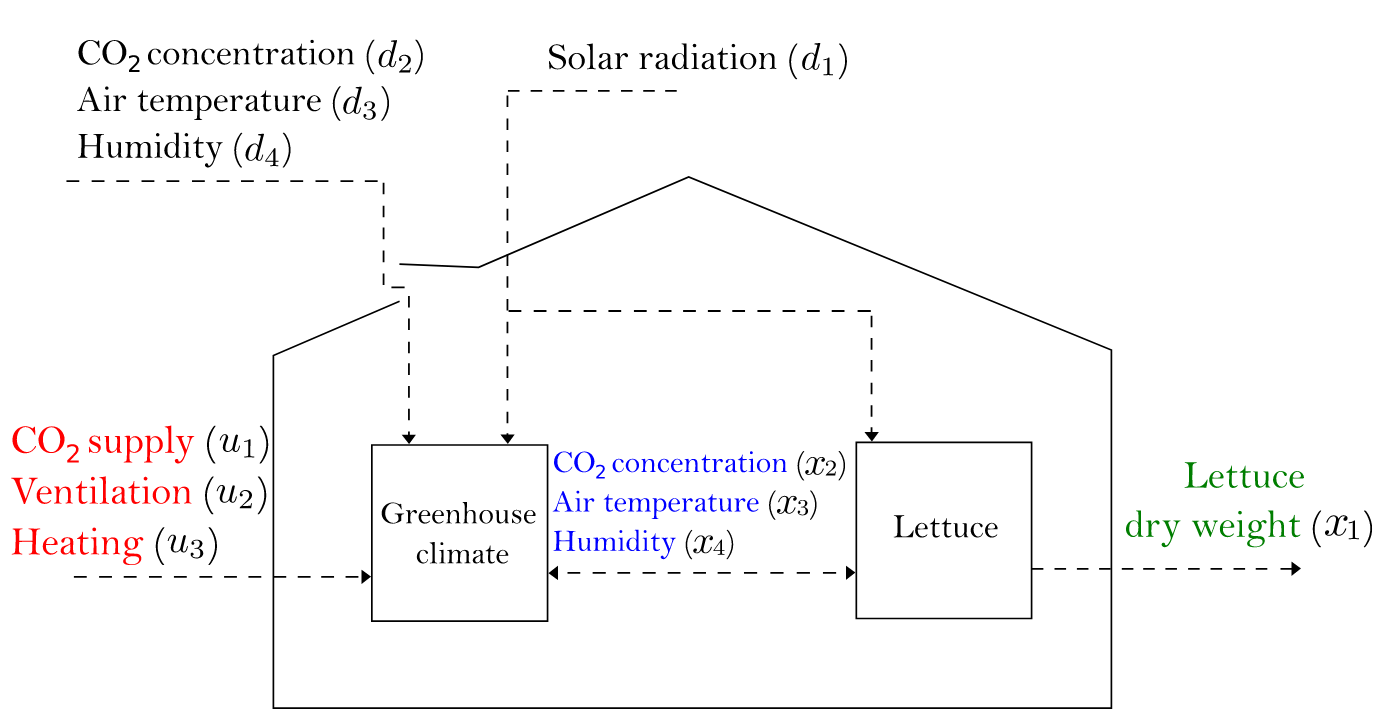
\includegraphics[width = \linewidth]{figures/van_henten_model.png}
	\caption{Graphical representation of greenhouse crop production \cite{hentenGreenhouseClimateManagement1994}}
	\label{fig:van_henten_model}
\end{figure}


\autoref{fig:van_henten_model} displays a graphical representation of the greenhouse model from the works of \citet{hentenGreenhouseClimateManagement1994} and has been used in previous works\cite{morcegoReinforcementLearningModel2023,lubbersAutonomousGreenhouseClimate2023, boersmaRobustSamplebasedModel2022}. The control inputs are highlighted in red, the states of the indoor climate in blue, the state of the crop in green and the external weather disturbances in black. The model was discretised with the fourth order Runge-Kutta Method with a sample period $\Delta t = 30$ min, resulting in the following system dynamics:
\begin{equation}\label{eq:greenhouse_model_discrete}
	\begin{aligned}
		& x(k+1) = f(x(k),u(k),d(k),p) \\
		& y(k) = g(x(k),p)
	\end{aligned}
\end{equation}
with discrete time $k \in Z^{0+}$, state variable $x(k) \in \mathbb{R}^4$, measurement $y(k) \in \mathbb{R}^4$, control input $u(k) \in \mathbb{R}^3$ and weather disturbance $d(k) \in \mathbb{R}^4$. The parameter $p \in \mathbb{R}^{28}$ represents all parameters used in the model, with $f(\cdot)$ and $g(\cdot)$ as the system's non-linear functions. The states of the system, control inputs, disturbances and outputs are described below.

\begin{equation}
	\begin{aligned}
		& x(k) = \begin{bmatrix}
			x_1 & x_{2} & x_3 & x_4
		\end{bmatrix}^T
		\\
		& u(k) = \begin{bmatrix}
			u_{1} & u_{2} & u_3
		\end{bmatrix}^T
		\\
		& d(k) = \begin{bmatrix}
			d_{1} & d_{2} & d_3& d_4
		\end{bmatrix}^T
		\\
		& y(k) = \begin{bmatrix}
			y_1 & y_{2} & y_3 & y_{4}
		\end{bmatrix}^T
	\end{aligned}
	\label{eq: model vectors}
\end{equation}

The measured output is essentially the same as the state of the system; however, the units of the indoor $C0_2$ density ($y_2$) and relative humidity ($y_4$) differ in that they report in units used in standard measurement sensors.

\begin{figure}[H]
	\centering
	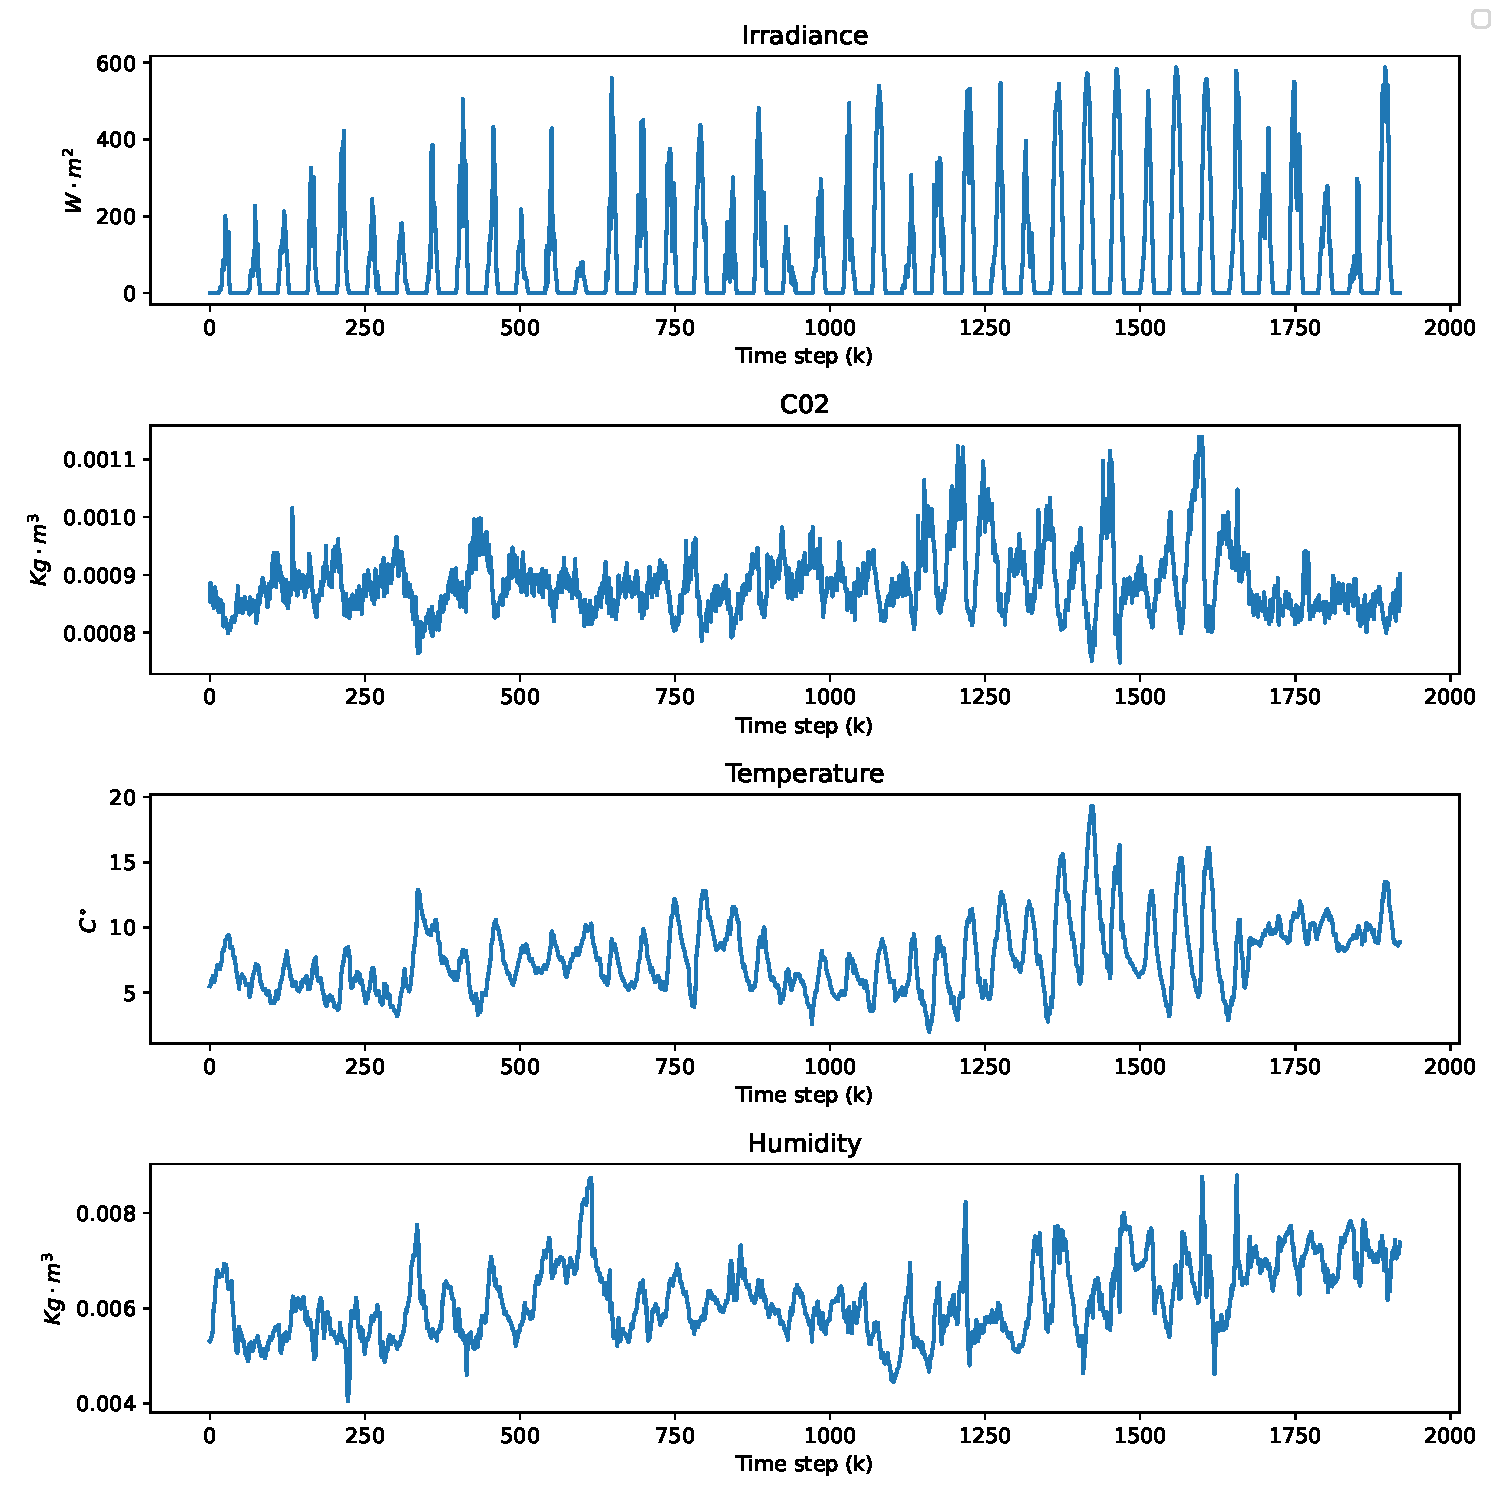
\includegraphics[width=\linewidth]{figures/weather_data_vertical.pdf}
	\caption{Weather Data}
	\label{fig:weather-data}
\end{figure}

The weather data for simulations and training was sourced from the Venlow Greenhouse in Bleiswijk, covering the period from January 30 to March 11, 2014. The weather is assumed to be deterministic and known at each time step. This dataset, shown in \autoref{fig:weather-data}, spans a 40-day growing period with a time step of 30 minutes, resulting in a total of 1920 time steps.



\subsection{Model Uncertainty}
As done in \cite{boersmaRobustSamplebasedModel2022, lubbersAutonomousGreenhouseClimate2023}, the source of uncertainty in the stochastic environment is modeled as parametric uncertainty, aiming to capture all the uncertainties in the greenhouse environment. The parameters of the environment are represented as uncertain with well-defined probabilistic properties. It is assumed that the uncertain parameters, $\hat{p}$, follow a uniform probabilistic distribution:

\begin{equation}
	\label{eq:uncertainty_model}
	\begin{aligned}
		\hat{p} \sim U(\mu_p, \delta_p)  
	\end{aligned}
\end{equation}

where $\mu_p$ is the mean value of the parameters and $\delta_p$ is expressed as a percentage such that the upper and lower bounds of the distribution is expressed as $p(1-\delta_p)$ and $p(1+\delta_p)$. This was done to guarantee that the sampled model parameters are always non-negative. Since all parameters are perturbed, including parameters of the output measurement equations, output noise is also introduced. Introducing this uncertainty results in the following system dynamics:

\begin{equation}\label{eq:greenhouse_model_discrete_uncertain}
	\begin{aligned}
		& \hat x(k+1) = f(\hat x(k),u(k),d(k),\hat p(k)) \\
		& \hat y(k) = g(\hat x(k),\hat p(k))
	\end{aligned}
\end{equation}

where the states and output measurements of the system are uncertain and $\hat{p}(k)$ denotes the uncertain parameters and is resampled at every time step.

\subsection{Optimization Goal}
To directly optimize the economic profit of the greenhouse, it is essential to maximize lettuce size while minimizing resource usage during its growth period, considering the pricing of energy and lettuce. This is referred to as the Economic Profit Indicator (EPI), and optimizing it forms the basis of the following optimization objective:

\begin{equation}\label{eq:epi}
	\min_{u_1,u_3}\sum_{k = t_s}^{t_f} (c_{p_1} \cdot u_1(k) + c_{p_2} \cdot u_3(k))\cdot \Delta t - c_{p_3} \cdot y_1(t_f)
\end{equation}

where $t_s$ denotes the start time of the growth period, $t_f$ the end time, $\Delta t$ the sample time interval,$c_{p1},c_{p2}$ the pricing coefficients of injecting $C0_2$, and heating, respectively and $c_{p3}$ as the price of lettuce. These pricing factors are shown in \autoref{tab:pricing_factors}. It is important to highlight that ventilation, such as opening windows, does not incur any costs and, therefore, does not have a pricing factor. $t_s$ and $t_f$ was selected so that the growing period is fixed at 40 days.\\
However, this optimization goal makes the reward incredibly sparse, making it difficult to optimize directly with both MPC and RL. Consequently, a stage cost received at every time interval is used, where the total sum of these stage costs throughout the growing period corresponds to the optimization objective in \autoref{eq:epi}. Therefore, the optimization goal that RL, MPC, and RL-MPC aim to optimize is:

\begin{subequations} \label{eq:optimisation-goal}
	\begin{align}
		& \min_{u_1,u_3} \sum_{k = t_s}^{t_f} \left[ l(y(k),u(k)) \right] \label{eq:stage-cost-epi} \\
		\text{s.t.} \quad 
		& \hat{x}(k+1) = f(\hat{x}(k), u(k), d(k), \hat{p}(k)), \label{eq:constraint-1} \\
		& \hat{y}(k) = g(\hat{x}(k+1), \hat{p}), \label{eq:constraint-dynamics} \\
		& -\delta u_{max} \leq u(k) - u(k-1) \leq \delta u_{max}, \label{eq:constraint-delta-u} \\
		& u_{\min} \leq u(k) \leq u_{\max}, \label{eq:constraint-u-limits} \\
		& x(k_0) = x_{k_0}. \label{eq:constraint-initial}
	\end{align}
\end{subequations}

where 
\begin{equation}
	l(y(k),u(k)) = (c_{p_1} \cdot u_1(k) + c_{p_2} \cdot u_3(k)) \cdot \Delta t  - c_{p_3} \cdot (y_1(k) - y_1(k-1))
\end{equation}
where the constraints are detailed below:
\begin{equation}\label{eq:constraints}
	\begin{aligned}
		&u_{min} = \begin{pmatrix}
			0&0&0
		\end{pmatrix}^T \\
		&u_{max} = \begin{pmatrix}
			1.2&7.5&150
		\end{pmatrix}^T	\\
		& \delta u_{max} = \frac{1}{10} u_{max}\\
		&y_{min} = \begin{pmatrix}
			0&500&10&0
		\end{pmatrix}^T \\
		&y_{max} = \begin{pmatrix}
			\infty&1600&20&100
		\end{pmatrix}^T	\\
	\end{aligned}
\end{equation}

The values in \autoref{eq:constraints} were obtained from typical horticultural practices and previous works \cite{boersmaRobustSamplebasedModel2022,morcegoReinforcementLearningModel2023,jansenOptimalControlLettuce2023}. 

\begin{table}[H]
	\centering
	\begin{tabular}{|c|c|c|}
		\hline
		\textbf{Symbol} & \textbf{Value} & \textbf{Units} \\
		\hline
		$c_{p_1}$ & $1.906\cdot 10^{-7} \times 10^{-4}$ & $ \text{\euro} \cdot mg^{-1}$ \\
		$c_{p_2}$ & $3.558 \times 10^{-8}$ & $ \text{\euro} \cdot J^{-1}$ \\
		$c_{p_3}$ & $22.285$ & $\text{\euro} \cdot kg^{-1}$ \\ 
		\hline
	\end{tabular}
	\caption{Pricing factors}
	\label{tab:pricing_factors}
\end{table}

\section{Problem Formulation}

\subsection{RL}
The Soft-Actor-Critic (SAC) algorithm is used in developing the Rl agent and is effective due to its ability to balance exploration and exploitation, handle continuous state and action spaces, and provide stable and efficient learning. SAC leverages both policy gradient methods and value function approximation, incorporating a value function to guide policy improvement and entropy regularization to encourage exploration. Moreover, such an actor-critic method provides both a policy (actor, $\pi (\cdot) $) and a critic (value function, $V_\pi (\cdot)$), that can be incorporated into the MPC's objective function. Interested readers are referred to \cite{SoftActorCriticSpinning} to learn how $\pi(\cdot)$ and $V_\pi(\cdot)$ are learned. It is noted that both the actor and critic are represented by neural networks.

\subsubsection{Agent Description}
The agent's description is influenced by its observation tuple (agent's state), its discount factor and reward function. The model of the environment is the same for all controllers used, i.e. RL, MPC and RL-MPC.

\begin{multline}\label{eq:obs-tuple}
	s(k) = (y_1(k),y_2(k),y_3(k),y_4(k), \\u_1(k-1), u_2(k-1), u_3(k-1), k, d(k))
\end{multline}

The agent's state, \autoref{eq:obs-tuple}, includes all the measurement outputs, the previous control inputs, the current time and weather disturbances. \\
The reward function is modelled after the optimisation goal, as defined in \autoref{eq:optimisation-goal}. State constraints cannot be directly imposed but can be indirectly incorporated by a penalty function in the reward function. It is common practice to impose a linear penalty function for state violations when learning a policy with RL. Therefore, the resulting reward function becomes:

\begin{multline}\label{eq:reward_fn}
	R(k)  =  - (c_{p_1} \cdot (u_1(k)) + c_{p_2} \cdot (u_3(k))) + \\ c_{p_3} \cdot (y_1(k)- y_1(k-1)) \\
	- (P_{c02} \cdot (y_2(k) ) + P_T \cdot (y_3(k)) + P_H \cdot (y_4(k)) )
\end{multline}

where the penalty terms $P_{c02},P_T,P_H$ are defined in \autoref{eq:penalty-terms}:

\begin{equation}\label{eq:penalty-terms}
	\begin{aligned}
		& P_{\text{CO2}} = 
		\begin{cases} 
			c_{p_{\text{CO2}}} \cdot (y_2(k) - y_2^{\text{max}}) & \text{if } y_2(k) > y_2^{\text{max}} , \\
			c_{p_{\text{CO2}}} \cdot (y_2^{\text{min}} - y_2(k)) & \text{if } y_2(k) < y_2^{\text{min}} , \\
			0 & \text{otherwise}
		\end{cases}
		\\
		& P_{T} = 
		\begin{cases} 
			c_{p_{T_{ub}}} \cdot (y_3(k) - y_3^{\text{max}}) & \text{if } y_3(k) > y_3^{\text{max}} , \\
			c_{p_{T_{lb}}} \cdot (y_3^{\text{min}} - y_3(k)) & \text{if } y_3(k) < y_3^{\text{min}} , \\
			0 & \text{otherwise}
		\end{cases}
		\\
		& P_{H} = 
		\begin{cases} 
			c_{p_{H}} \cdot (y_4(k) - y_4^{\text{max}}) & \text{if } y_4(k) > y_4^{\text{max}} , \\
			c_{p_{H}} \cdot (y_4^{\text{min}} - y_4(k)) & \text{if } y_4(k) < y_4^{\text{min}} , \\
			0 & \text{otherwise}
		\end{cases}
		\\
	\end{aligned}
\end{equation}

The penalty constants $c_{p_{CO_2}}, c_{p_{T_{ub}}},c_{p_{T_{lb}}},c_{p_{H}}$ were found empirically in \citet{jansenOptimalControlLettuce2023} to effectively account for deviations from desired states and their impact on the economic benefit. The penalty constants and their respective units are displayed in \autoref{tab:pen-constants}.\\
To accommodate for the control input constraints (\autoref{eq:constraint-u-limits}, \autoref{eq:constraint-delta-u}), the actor ($\pi(\cdot)$) has a continuous action space, denoted as \( \mathcal{A} \),  and is defined as \( \mathcal{A} = [-1, 1]^3 \), where \( \mathcal{A} \subseteq \mathbb{R}^3 \). The agent’s action, denoted as  $a(k) = \pi (s(k))$, where $a \in \mathcal{A}$, is regarded as a modification to the control input. Consequently, the current control input can be determined as follows:
$$
u(k) = \max(u_{\min}, \min(u(k-1) + a(k) \cdot \delta u_{\max}, u_{\max}))
$$

where $\delta u_{max}(k),u_{min}, u_{max}$ are defined in \autoref{eq:constraints}. 


\begin{table}[h]
	\centering
	\begin{tabular}{|>{\bfseries}l|c|c|}
		\hline
		\textbf{Parameter} & \textbf{Value} & \textbf{Units} \\
		\hline
		$c_{p_{\text{CO2}}}$ & $\frac{10^{-3}}{20}$ & \euro$\cdot (ppm \cdot m^2)^{-1}$ \\
		$c_{p_{T_{ub}}}$ & $\frac{1}{200}$ & \euro$\cdot (C^{\circ} \cdot m^2)^{-1}$ \\
		$c_{p_{T_{lb}}}$ & $\frac{1}{300}$ & \euro$\cdot (C^{\circ} \cdot m^2)^{-1}$ \\
		$c_{p_{H}}$ & $\frac{1}{50}$ & \euro$\cdot (RH_{\%} \cdot m^2)^{-1}$ \\
		$y_2^{max}$ & $1600$ & ppm \\
		$y_2^{min}$ & $500$ & ppm \\
		$y_3^{max}$ & $20$ & $C^{\circ}$ \\
		$y_3^{min}$ & $10$ & $C^{\circ}$ \\
		$y_4^{max}$ & $100$ & $RH_{\%}$ \\
		$y_4^{min}$ & $0$ & $RH_{\%}$ \\       
		\hline
	\end{tabular}
	\caption{Penalty Constants}
	\label{tab:pen-constants}
\end{table}

\subsubsection{Agent Training}
Stable baselines 3 (SB3) \cite{raffinStableBaselines3ReliableReinforcement2021} was used to facilitate the development and training of the SAC algorithm. The final hyper-parameters and actor-critic network structures are posted in \autoref{tab:hyper-params} and were found empirically. The defaults provided by SB3 are used for hyper-parameters that are not reported. All random generators in the experiments were seeded with a value of 4 to ensure reproducibility of the results.

\begin{table}[H]
	\centering
	\begin{tabular}{|>{\bfseries}l|c|}
		\hline
		\textbf{Parameter} & \textbf{Value} \\
		\hline
		Training episodes & $100$  \\
		Warm-up episodes &  $9$ \\
		Hidden layers & $2$ \\
		Neurons per hidden layer & $128$ \\
		Batch size & $1024$ \\
		Learning rate & $5 \cdot 10^{-3}$ \\
		Buffer size & $100000$ \\
		Discount Factor & $0.95$ \\
		Activation Function & ReLu \\
		\hline
	\end{tabular}
	\caption{Hyper-parameters}
	\label{tab:hyper-params}
\end{table}

In RL problems with a fixed, long-term horizon, a discount factor ($\gamma$)
of 1 is often desired. This setting ensures that the RL agent's prediction horizon covers the entire growing period, allowing the critic to evaluate and retain information about the full state trajectory and the actor to make long-term decisions. Consequently, the critic can provide accurate value estimations based on long-term outcomes.\\
However, using $\gamma = 1$ can make it challenging to find a competitive policy. To address this, a lower discount factor was employed, which facilitated the discovery of a more effective policy. Nevertheless, this adjustment means that the critic's value estimates are based on discounted returns rather than the true long-term expected return.

To reconcile these issues, we trained a separate critic with $\gamma = 1$ on the fixed policy obtained through SAC. This approach leverages the advantages of a practical policy while ensuring that the critic provides accurate value estimations over the entire trajectory.


\subsubsection{Value Function Learning}
In order to train a value function, multiple trajectories are sampled and for each state visited, the expected return is calculated as per \autoref{eq:return_function}. 

\begin{equation}
	\begin{aligned}
		G_t  = R_{t+1} + R_{t+2} + R_{t+3} + \dots + R_{T} = \sum_{k=0}^TR_{t+k+1}
	\end{aligned}
	\label{eq:return_function}
\end{equation}

All initial states and inputs were uniformly sampled around a region of the nominal trajectory at time $k$. Initial states and inputs were sampled from $\hat{\mathbb{X}^4}$ and $\hat{\mathbb{U}^3}$ and the initial time step $k$ is uniformly sampled across the entire time horizon as shown in \autoref{eq:TR-sample-space}.


\begin{equation}\label{eq:TR-sample-space}
	\begin{split}
		\hat{\mathbb{X}}^4 &= \{ (\hat{x}_1, \hat{x}_2, \hat{x}_3, \hat{x}_4) \mid\ \hat{x}_1 \in [\hat{x}_{1\min}(x_{1_k}), \hat{x}_{1\max}(x_{1_k})], \\
		&\quad \hat{x}_2 \in [\hat{x}_{2\min}(x_{2_k}), \hat{x}_{2\max}(x_{2_k})], \\
		&\quad \hat{x}_3 \in [\hat{x}_{3\min}(x_{3_k}), \hat{x}_{3\max}(x_{3_k})], \\
		&\quad \hat{x}_4 \in [\hat{x}_{4\min}(x_{4_k}), \hat{x}_{4\max}(x_{4_k})] \} \\
		\hat{\mathbb{U}}^3 &= \{ (\hat{u}_1, \hat{u}_2, \hat{u}_3) \mid\ \hat{u}_1 \in [\hat{u}_{1\min}(u_{1_k}), \hat{u}_{1\max}(u_{1_k})], \\
		&\quad \hat{u}_2 \in [\hat{u}_{2\min}(u_{2_k}), \hat{u}_{2\max}(u_{2_k})], \\
		&\quad \hat{u}_3 \in [\hat{u}_{3\min}(u_{3_k}), \hat{u}_{3\max}(u_{3_k})] \} \\
		& k \sim U(0,1919)  \\
	\end{split}
\end{equation}

where the minimum and maximum limits are calculated as per \autoref{eq:min-max-tr-sample-space}

\begin{equation}\label{eq:min-max-tr-sample-space}
	\begin{aligned}
		&\hat{z}_{min} = z_k \cdot (1-\sigma)\\
		&\hat{z}_{max} = z_k \cdot (1+\sigma)
	\end{aligned}
\end{equation}

which represent the minimum and maximum range of the sample state space for a specific state and input where ${z}_{k}$ represents the nominal trajectory, $\sigma$ denotes the desired spread of sampled initial states, which is expressed as a percentage. Given that the actor was found to compute a control action in $0.2 ms$, 1000 trajectories were sampled to achieve appropriate coverage of state and input spaces.
A neural network  was trained with inputs as the state, $s_k$, and labels as the total return,$G_t$ and the loss function in \autoref{eq:vf_tr_loss} is minimised with the Adam optimiser:
\begin{equation}
	\label{eq:vf_tr_loss}
	L(\phi, \mathcal{D}) =   V_{\phi}(s_k) - \mathbb{E}(G_t(s_k))
\end{equation}
where $V_{\phi}$ is the function approximator with weights $\phi$ and $G_t(s_k)$ is the total return of state $s_k$. Parameters include a 2 hidden layer network with 128 neurons per layer, a $1\cdot 10^{-3}$ learning rate and a batch size of 1024 trained on 200 epochs. Initially,  input, $s(k)$, for the value function was the same as that used by the RL agent (\autoref{eq:obs-tuple}). However, it was discovered that the expected return of a state could be reasonably estimated using only the current dry mass and time. This simplification also reduced the non-linearity of the neural network, making it suitable for use in the MPC formulation. While training on the full state of the agent allowed for more accurate predictions of the expected return, the increased non-linearity of the neural network adversely affected the MPC optimizer when integrated as a cost function.


\subsection{MPC}
Similarly to the RL agent, the MPC aims to optimize the objective function defined in \autoref{eq:optimisation-goal}. To facilitate direct comparisons between RL, MPC, and RL-MPC, the same linear penalty constraints, as described in \autoref{eq:penalty-terms}, were used in the form of slack variables. Therefore, the following optimization goal is solved at every time step:
\begin{equation} \label{eq:mpc_ocp}
	\begin{aligned}
		&\min_{u(k),x(k)}  \sum_{k = k_0}^{k_0 + N_p-1} \Bigg[ l(y(k),u(k)) + \sum_{i = 1}^6 s_i(k) \Bigg]  \\
		&\text{s.t.} \quad x(k+1) = f(x(k), u(k), d(k), \mu_p), \\
		 &y(k) = g(x(k+1), \mu_p), \\
		 &-\delta u_{max} \leq u(k) - u(k-1) \leq \delta u_{max}, \\
		 &u_{\min} \leq u(k) \leq u_{\max}, \\
		 &x(k_0) = x_{k_0}, \\
		 &s_i(k) \geq 0, \\
		 &s_1(k) \geq c_{p_{C02}} \cdot (y_2^{min} - y_2(k)), \\& s_2(k) \geq c_{p_{C02}} \cdot (y_2(k) + y_2^{max}), \\ 
		 &s_3(k) \geq c_{p_{T_{lb}}} \cdot (y_3^{min} - y_3(k)),\\& s_4(k) \geq c_{p_{T_{ub}}} \cdot (y_3(k) + y_3^{max}), \\ 
		 &s_5(k) \geq c_{p_{H}} \cdot (y_4^{min} - y_4(k)),\\& s_6(k) \geq c_{p_{H}} \cdot (y_4(k) + y_4^{max}).
	\end{aligned}
\end{equation}

The policy generated by the MPC is denoted $\kappa(x,u,d,p)$ where the optimal control action to take at time $k$ is

\begin{equation}\label{eq:mpc_policy_notation}
	u_k^* = \kappa(x_k,u_{k-1}^*, d_k, \mu_p)
\end{equation}

The open-source software CasADi  \cite{anderssonCasADiSoftwareFramework2019} and solver IPOPT \cite{wachterImplementationInteriorpointFilter2006} are used in Python to solve \autoref{eq:mpc_ocp}.


\subsection{RL-MPC}
According to \citet{ellisTutorialReviewEconomic2014} and \citet{amritEconomicOptimizationUsing2011}, an EMPC without a terminal constraint and terminal cost function faces challenges in proving performance and stability guarantees. Specifically, \citet{ellisTutorialReviewEconomic2014} asserts that a terminal point constraint is necessary to ensure closed-loop performance. Additionally, \citet{amritEconomicOptimizationUsing2011} argues that a terminal cost function with a terminal region constraint is superior to a terminal point constraint, as it enlarges the feasible set of initial conditions and may enhance closed-loop performance. However, identifying suitable terminal constraints and cost functions is challenging. This study aims to determine whether an RL agent can provide these elements. Furthermore, from an RL perspective, the learned value function is only an approximation. When used in MPC, this value function is effectively unrolled, executing value iterations, which can lead to an improved policy compared to the original policy that generated the value function.

The solution to the OCP in \autoref{eq:mpc_ocp} at time $k$ can be denoted as:

\begin{equation}\label{eq:sol-mpc-ocp}
	\begin{aligned}
		&\mathbf{x}_{k|k} = [x_{k|k},x_{k_+ 1|k},x_{k + 2|k}, ...,x_{k + N_p|k}]^T \\ 
		&\mathbf{u}_{k|k} = [u_{k|k},u_{k + 1|k}, ...,u_{k + N_p-1|k}]^T \\
	\end{aligned}
\end{equation}

Where the initial guess generated by the RL agent at time $k$ is denoted as:

\begin{equation}\label{eq:initial-guess}
	\begin{aligned}
		&\tilde{\mathbf{x}}_{k|k} = [\tilde{x}_{k|k},\tilde{x}_{k+1|k},...,\tilde{x}_{k + N_p|k}]^T \\ 
		&\tilde{\mathbf{u}}_{k|k} = [\tilde{u}_{k|k},\tilde{u}_{k + 1|k},...,\tilde{u}_{k + N_p - 1|k}]^T\\ 
	\end{aligned}
\end{equation}

such that

\begin{equation}\label{eq:horizon_extension}
	\begin{aligned}
		&\tilde{\mathbf{x}}_{k|k} = [\mathbf{x}_{k|k-1}, \\ & f(x_{k-1 + N_p|k-1}, \pi(x_{k-1 + N_p|k-1}), d_{k+Np|k},p)]^T \\ 
		&\tilde{\mathbf{u}}_{k|k} = [\mathbf{u}_{k|k-1},\pi(x_{k-1 + N_p|k-1})]^T\\
	\end{aligned}
\end{equation}

\autoref{eq:horizon_extension} takes the previous time steps solution, shifts it in time and uses the policy $\pi(\cdot)$, as provided by the actor, to calculate the optimal action and resulting state to take at the last time step. This method can be interpreted as extending the MPC's horizon. It must be noted that, for the first time step, $k=0$, the intial guess is generated by unrolling the RL policy for the entire horizon. Based on prior analyses, generating these initial guesses is extremely fast. Furthermore, since it comes from a policy comparable to the MPC’s which optimises the same goal, these initial guesses can be used for more than just initial guesses, but also to generate terminal constraints. The terminal region is defined as:

\begin{equation}\label{eq:terminal-region}
	\begin{aligned}
		& (1-\delta_T)\tilde{x}_{k+Np|k} \leq x_{k+Np|k} \leq (1+\delta_T)\tilde{x}_{k+Np|k}\\
		&(1-\delta_T)\tilde{u}_{k+Np-1|k} \leq u_{k+Np-1|k} \leq (1+\delta_T) \tilde{u}_{k+Np-1|k}\\
	\end{aligned}
\end{equation}

The terminal cost function takes the form of the value function learned $V_\phi$ and therefore, the resulting RL-MPC OCP is defined as:

\begin{equation} \label{eq:rl-mpc-ocp}
	\begin{aligned}
		\min_{u(k),x(k)} & \sum_{k = k_0}^{k_0 + N_p-1} l(u(k), y(k)) - V_{\phi}(y_1(k_0+N_p), k_0+N_p) \\
		\text{s.t.} \quad & x(k+1) = f(x(k), u(k), d(k), p), \\
		& y(k) = g(x(k+1), p), \\
		& -\delta u \leq u(k) - u(k-1) \leq \delta u, \\
		& u_{\min} \leq u(k) \leq u_{\max}, \\
		& x(k_0) = x_{k_0}, \\
		& \tilde{\mathbf{x}}_{k|k} = [\mathbf{x}_{k|k-1}, f(x_{k-1 + N_p|k-1}, \pi(x_{k-1 + N_p|k-1}), d_{k+Np|k}, p)]^T, \\
		& \tilde{\mathbf{u}}_{k|k} = [\mathbf{u}_{k|k-1}, \pi(x_{k-1 + N_p|k-1})]^T, \\
		& (1-\delta_T)\tilde{x}_{k+Np|k} \leq x_{k+Np|k} \leq (1+\delta_T)\tilde{x}_{k+Np|k}, \\
		& (1-\delta_T)\tilde{u}_{k+Np-1|k} \leq u_{k+Np-1|k} \leq (1+\delta_T)\tilde{u}_{k+Np-1|k}.
	\end{aligned}
\end{equation}


This implementation was investigated to determine whether RL could provide an adequate terminal region and cost function to improve the original EMPC's performance, thereby producing a high-performing EMPC, also known as RL-MPC. The goal was to achieve these improvements for shorter prediction horizons and to transfer knowledge of the system's uncertainty to enhance the EMPC's ability to handle such uncertainties. In conjuction with Casadi and IPOPT, the open-source software L4Casadi \cite{salzmannLearningCasADiDatadriven2023,salzmannRealtimeNeuralMPCDeep2023} was used to develop the RL-MPC framework and solve \autoref{eq:rl-mpc-ocp}.


\section{Simulation Results}
The simulation results are categorized into two components: the nominal (deterministic) environment and the stochastic environment.


In a nominal environment with no parameter deviation ($\delta = 0\%$), RL, MPC, and RL-MPC algorithms were simulated and trained using a deterministic prediction model($\hat{p}(k) = \mu_p$). This setup ensures that repeated simulations yield identical results. The nominal environment was crucial for developing the RL-MPC algorithm and evaluating the effectiveness of RL in providing useful terminal constraints and cost functions. Additionally, it served as the basis for generating the nominal trajectories for states and inputs.

In the stochastic environment, we test three levels of uncertainty: $\delta = 5\%$, $10\%$, and $20\%$. For these cases, MPC and RL-MPC continue to use a deterministic prediction model. However, three RL agents are trained, each specifically for one level of uncertainty. The stochastic environment is used to evaluate whether RL can impart its knowledge of the system's uncertainty to the EMPC, enabling the resulting RL-MPC algorithm to better handle the present uncertainty. Although the RL-MPC formulation relies on a deterministic prediction model, it leverages the RL agents’ knowledge of uncertainties. For each level of uncertainty, the RL-MPC’s initial guesses, terminal constraints, and terminal cost function are derived from the RL agent trained for that specific uncertainty level. Finally, prediction horizons of 1-6 hours were tested for the MPC and RL-MPC. Lastly, modification to the RL-MPC is made to ease the computational burden and tested against the original RL-MPC. For all simulations it was decided to have $\epsilon = 5\%$.

\subsubsection{Performance Metrics}
The performance metrics include the final cumulative reward achieved over the simulation period. This reward is the sum of stage costs, which encompasses \autoref{eq:optimisation-goal}, along with penalties for state and output violations. In other words, the sum of stage costs of \autoref{eq:reward_fn} or \autoref{eq:mpc_ocp}. Performance metrics for the nominal case will also include the computational time of each algorithm. For the stochastic setting, the performance metrics are detailed by including the mean final cumulative reward, averaged across 30 simulation runs, as well as the variance of the final cumulative reward.\\
To note, time series plots of the evolution of the system's states and inputs are not shown, since they are similar to those posted in \cite{morcegoReinforcementLearningModel2023, jansenOptimalControlLettuce2023, boersmaRobustSamplebasedModel2022}.

\subsection{Deterministic}
 \autoref{fig:rl-mpc-nominal} displays the performance and the computational time of the RL, MPC and the RL-MPC algorithms with various prediction horizons. 
\begin{figure}[h]
	\centering
	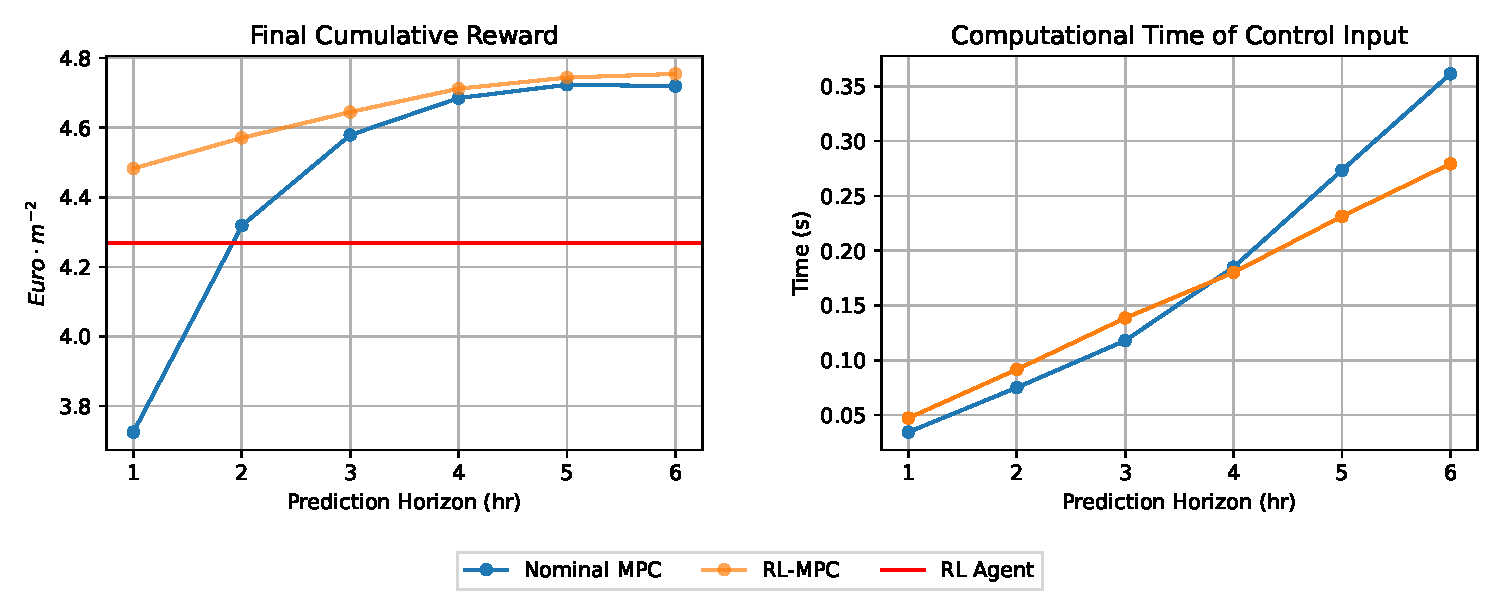
\includegraphics[width=\linewidth]{figures/rl_mpc_impl_final_research.pdf}
	\caption{Comparison of RL, MPC and RL-MPC on the nominal environment}
	\label{fig:rl-mpc-nominal}
\end{figure}
 It is clear that MPC is not myopic as previously thought. It noticeable outperforms the RL agent, with increased performance as prediction horizons increases, however; naturally, the computational time also increases. One could argue that it might not be necessary to introduce terminal constraints and a cost function from RL since performance of the EMPC is satisfactory. However, introducing these constraints and cost function boosts performance further across all prediction horizons, and significantly so at lower prediction horizons. Although the addition of a neural network as a cost function increases the computational time, it was found that the addition of the terminal constraints significantly lowers it to the point where the complete RL-MPC algorithm is faster the original MPC at higher prediction horizons. At lower prediction horizons, specifically 1 and 2 hours, the trade off between increased performance and increased computational costs is clearly in favour of increased performance. It is important to note that these terminal constraints and cost function are provided by an RL policy that performs considerably worse than MPC; however, they still visibly improve the RL-MPC performance. This demonstrates the importance of providing an EMPC with appropriate terminal constraints and cost functions to achieve superior performance.\\  
Lastly, one could argue that since the computational speeds are relatively fast compared to the control time interval (sub-second computational speeds versus a 30-minute interval), the prediction horizon can be increased until performance requirements are met. However, this model of the greenhouse system is relatively simple. More complex models may not offer the same flexibility in extending the prediction horizon.

\subsection{Stochastic}
Stochastic results are presented in \autoref{fig:rl-mpc-stochastic} and \autoref{fig:rl-mpc-stochastic-10}
\begin{figure}[h]
	\centering
	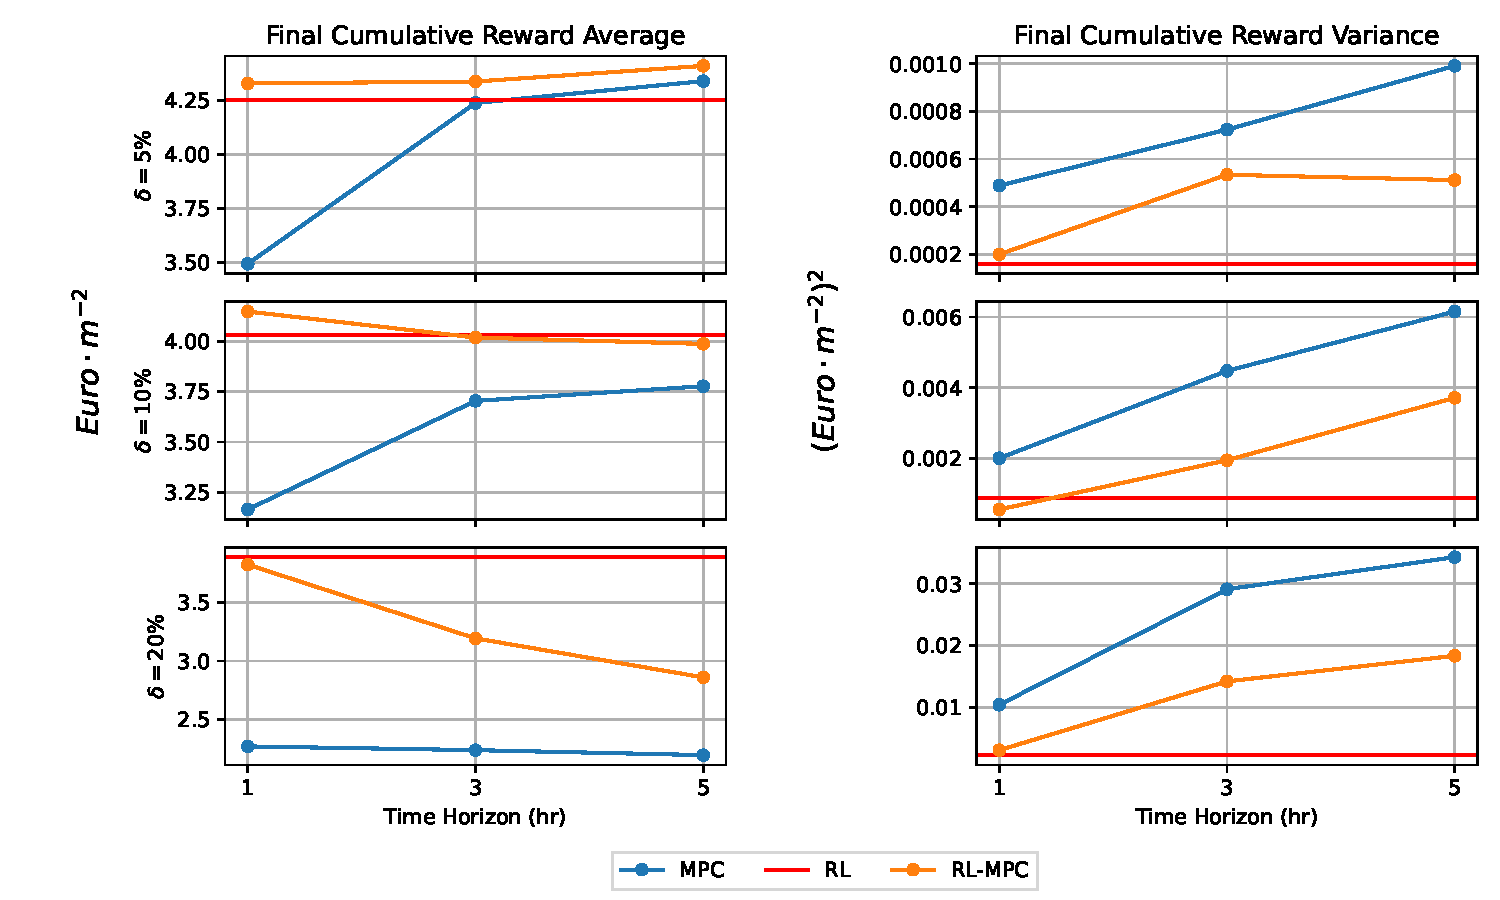
\includegraphics[width=\linewidth]{figures/stochastic_rl_vs_mpc_impl3.eps}
	\caption{Comparison of RL, MPC and RL-MPC across all prediction horizons}
	\label{fig:rl-mpc-stochastic}
\end{figure}
\autoref{fig:rl-mpc-stochastic} presents the findings of RL, MPC, and RL-MPC in a stochastic environment with varying levels of uncertainty across 1, 3, and 5-hour prediction horizons. It is evident that as uncertainty increases, RL outperforms MPC due to RL's ability to learn and manage uncertainty. Moreover, increasing the prediction horizon for MPC under higher uncertainty yields diminishing performance returns. The variance of RL is significantly lower than that of MPC, with the difference increasing as uncertainty rises.\\
In the case of RL-MPC, similar to the nominal scenario, at low uncertainties, RL-MPC outperforms both MPC and RL in terms of final mean cumulative reward. For all levels of uncertainty, RL-MPC noticeably outperforms MPC in both cumulative reward and variance across all prediction horizons. This demonstrates that the terminal constraints and cost function provided by RL impart knowledge of the uncertainty in the environment. Although RL still outperforms RL-MPC at higher levels of uncertainty, RL-MPC performs substantially better than the original EMPC.

Often, a conservative estimate of the uncertainty in the environment is used to develop a controller. Hence, \autoref{fig:rl-mpc-stochastic-10} includes the performance of an RL agent trained on data with $\delta_p = 10\%$, the RL-MPC algorithm that uses this agent, and the original MPC tested across three different uncertainty levels. The prediction horizon for the MPC and RL-MPC was fixed at 3 hours.

\begin{figure}[h]
	\centering
	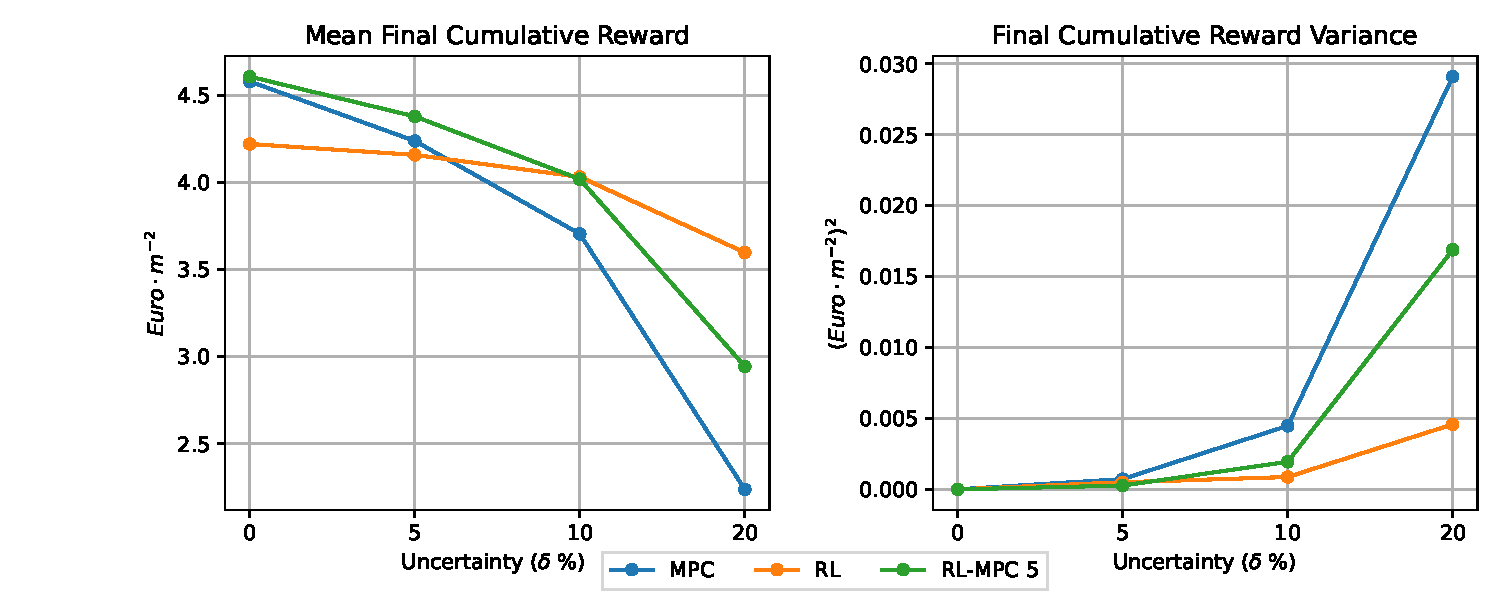
\includegraphics[width=\linewidth]{figures/stochastic_realife.eps}
	\caption{Comparison of RL, MPC and RL-MPC developed at $\delta_p = 10\%$}
	\label{fig:rl-mpc-stochastic-10}
\end{figure}

The superiority of the RL-MPC controller over both MPC and RL is illustrated in \autoref{fig:rl-mpc-stochastic-10}, particularly regarding mean final cumulative reward at low uncertainty levels. This trend persists until uncertainty reaches a threshold where MPC's performance noticeably declines, which negatively affects the RL-MPC's performance. Despite this, RL-MPC consistently outperforms MPC, showing a less severe performance drop as uncertainty increases. The RL agent remains the best performer under high uncertainty. \autoref{fig:rl-mpc-stochastic-10} suggests that equipping an EMPC with terminal constraints and a cost function generated by an RL agent trained on stochastic data enhances the EMPC's understanding and management of system uncertainty. Essentially, this approach makes the EMPC more robust against noise without sacrificing performance at lower uncertainty levels, and even enhances it.


\subsection{Speedup}
Although the original MPC and RL-MPC offer real-time computational speeds across all prediction horizons, RL-MPC may not be real-time for more complex systems due to the added computational burden from the neural network used as a cost function. Simplifying the neural network architecture and using approximations can help address this issue. While it was found that reducing the network size can improve computational speeds without performance loss, the focus here is on using Taylor approximations of the neural network around the terminal guess provided by RL. The results of this approach are shown in \autoref{fig:rl-mpc-speedup}.

\begin{figure}[h]
	\centering
	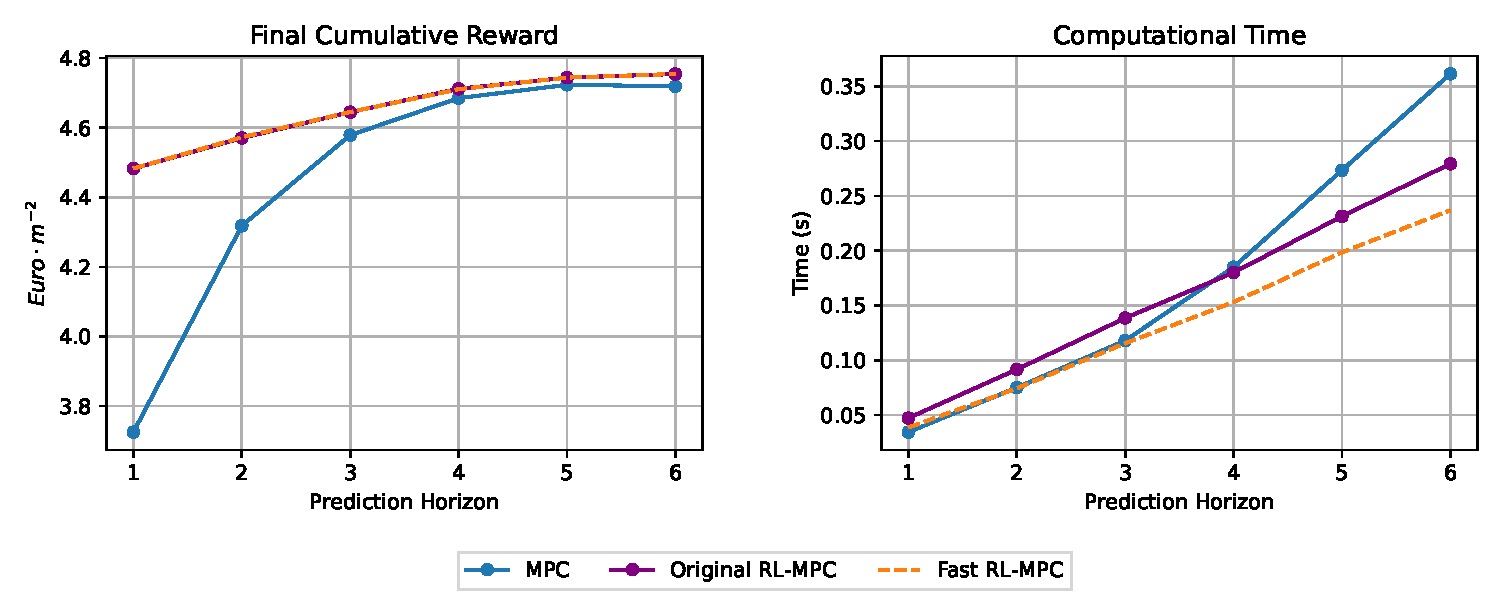
\includegraphics[width=\linewidth]{figures/final_speed_up.pdf}
	\caption{Fast RL-MPC}
	\label{fig:rl-mpc-speedup}
\end{figure}


It was found that a second-order Taylor approximation did not provide any advantage over a first-order approximation and hence not shown here. \autoref{fig:rl-mpc-speedup} illustrates that the first-order Taylor approximation results in a substantial increase in computational speeds without sacrificing performance, making the RL-MPC algorithm as fast as MPC at shorter prediction horizons. This approach is both simple and highly effective for making the RL-MPC algorithm faster.


\chapter{Discussion and Conclusion}
\label{chapter:conclusion}

This thesis proposed an RL-MPC algorithm to assess the performance gains compared to the standalone RL and MPC controllers on a greenhouse environment. Two similar performing policies were created with RL and MPC for a deterministic and stochastic environment. The RL-MPC algorithm was developed in the deterministic environment by testing various combinations of the two controllers to determine whether RL is able to provide the RL-MPC useful information in deciding control inputs. The resulting RL-MPC was tested on a stochastic environment to determine whether RL can impart knowledge of the uncertainty to the RL-MPC framework. Lastly, modifications were investigated that could reduce the computational demand of the RL-MPC controller. This chapter assessed the research questions asked at the beginning of this thesis and drew final conclusions about the RL-MPC controllers, with recommendations for future research.

\section{Conclusion}
This thesis aimed to answer two research questions, namely:

\begin{itemize}[itemsep=7pt] % Adjust the value of itemsep to change spacing
	\item \textit{How does the economic performance of the RL-MPC algorithm compare to the standalone RL and MPC algorithms?} 
	
	\begin{itemize}
		\item \textit{Deterministic Environment:} 
		\\The results presented in this thesis demonstrate that the RL-MPC algorithm greatly enhances economic performance compared to the standalone RL and MPC algorithms. The MPC policy outperformed the policy generated from RL in this particular setting, and its superiority was further enhanced with an increase in the prediction horizon. While the MPC's performance could be deemed satisfactory, the RL-MPC algorithm demonstrated superior economic performance across all prediction horizons of the MPC, with particularly notable results at shorter prediction horizons. Results show a $24\$$ increase in performance over MPC and a $5\%$ over RL at a 1 hour prediction horizon with greater performance over RL over and less performance over MPC at longer prediction horizons. This concludes that even a worse-performing policy (in this case, the RL agent) can provide useful information to an MPC through terminal constraints generated by the actor and a value function as a cost function.
		
		\item \textit{Stochastic Environment:} 
		\\	
		Evidence demonstrated that RL exhibits a superior ability to manage uncertainty when trained with corresponding stochastic data compared to MPC. However, since the MPC was not adjusted to address this uncertainty, RL outperformed MPC, especially under high uncertainty conditions. This thesis aimed to demonstrated that RL can transfer knowledge of this uncertainty to MPC through the development of the RL-MPC framework. The developed RL-MPC algorithm was shown to achieve superior performance compared to both RL and MPC controllers under low uncertainty, similar to the deterministic scenario. Although RL-MPC's performance is hindered by the subpar performance of MPC in high uncertainty settings, it remains more robust than MPC with a slower decline in performance as uncertainty is increased. While RL-MPC continues to surpass MPC in performance, it faces challenges in achieving the same level of performance as RL in situations with high levels of uncertainty.
	\end{itemize}
	
\end{itemize}


\begin{itemize}[itemsep=7pt] % Adjust the value of itemsep to change spacing
	\item \textit{What modifications and/or approximations can be employed to reduce the computational time of the RL-MPC algorithm?}
	\\Additional modifications can be made to reduce the computational burden of the RL-MPC algorithm. These modifications include training a simpler neural network with fewer neurons and hidden layers and using a first- and second-order Taylor approximation of the neural network around the terminal guess. It was shown that the computational demand and performance depend on the size and complexity of the neural network; however, no direct relationship was noticed between reduced computational burden and size of the neural network. However, it was found that it is possible to use a  simpler neural network for decreased computational times with no impact on performance. Moreover, it was shown that using both a first- and second-order Taylor approximation noticeably decreased computational burden while resulting in very little to no performance losses. The combination of both techniques yielded an RL-MPC controller that exhibited computational times significantly faster than those of the original RL-MPC while preserving its original performance. Furthermore, the achieved computational times were similar to those of MPC for short prediction horizons and faster for longer prediction horizons. 
\end{itemize}

The superiority of the RL-MPC controller over its standalone counterparts is evident, with the most significant performance enhancement achieved by incorporating a terminal region constraint. While incorporating a suitable value function does enhance performance, it also substantially increases computational demand. In contrast, the terminal region constraint not only enhances performance but also decreases computational load. It should be acknowledged that the greenhouse model used in this thesis is relatively uncomplicated. Including the value function may produce more significant benefits in larger and more complex systems.

The computational burden of the RL-MPC algorithm can be similarly argued. Despite the RL-MPC algorithm demonstrating relatively fast computational speeds, even outperforming MPC at long prediction horizons, one might question the need for modifications to enhance its speed further. The RL-MPC algorithm provides real-time control for a relatively simple non-linear system. However, achieving real-time control for much larger systems may become challenging and essential for performance. Moreover, the modifications are simple to incorporate and do not impact performance, so there is no reason not to implement them.

It was noted in this thesis that training an RL policy was significantly more difficult and time-consuming than generating a policy using MPC. Thus, MPC would likely be preferred in real-world applications, if a model is readily available. However, results show that even a suboptimal RL policy can be integrated into MPC to create an RL-MPC algorithm that surpasses MPC's performance and increases robustness to uncertainty for all prediction horizons. This highlights the importance of integrating the two methods.


\section{Recommendations and Future Work}

\begin{itemize}
	\item \textit{Improvements to the RL algorithm}
	\\Further study into the hyper-parameters of the RL agent may be necessary to generate an RL policy capable of outperforming MPC in a deterministic environment. This could help determine how an increase in RL policy performance can affect the RL-MPC performance.  Moreover, different RL algoritms such as PPO, TRPO, or other advanced optimization algorithms  can be used to improve the policy's performance. Furthermore, in learning a value function, it is important to note that neural networks are not the only non-linear function approximators available. Other forms, such as radial basis functions or Gaussian processes, may be more suitable for effectively learning a value function for the dynamics of the greenhouse and may be more stable (i.e. display a lower degree of non-linearity) when implementing it into the RL-MPC framework. An in-depth investigation is necessary to determine which function approximator is most suitable.
	
	\item \textit{Improvements to the MPC formulation}
	\\In the stochastic environment, RL outperforms MPC because it is provided with information about the uncertainty present, whereas MPC is not. This was done to assess whether RL can transfer its knowledge of this uncertainty into the RL-MPC framework through a terminal region constraint and a value function. However, estimation techniques such as Moving Horizon Estimation (MHE) are commonly used in MPC to mitigate output noise. Additionally, stochastic MPC controllers, like those addressing parametric uncertainty, can significantly enhance MPC performance in a stochastic environment. Therefore, a study incorporating these techniques into the RL-MPC framework should be performed to examine potential performance gains and improved robustness.
	
	Finally, it was demonstrated that the performance degradation of the MPC and RL-MPC controllers in a stochastic environment was primarily due to the increase in constraint violations. Since soft constraints were imposed in this thesis, it may be beneficial to impose hard constraints and investigate their impact on both MPC and RL-MPC. This would help determine whether RL can continue to provide valuable information to RL-MPC for performance improvements.
	
	
	\item \textit{Improvements to the model}
	\\A more accurate uncertainty model could better predict the controllers' behavior in a realistic environment by accounting for uncertainty in energy costs, lettuce prices, and weather. Additionally, the studies performed in this thesis could be conducted in a more complex environment, such as in \citet{GreenLightOpenSource2020}, to better determine the real-world applicability of RL-MPC. Further research could involve training an RL policy on the more complex model and implementing RL-MPC on the simplified model, as this would likely be done in practice. Moreover, RL and MPC could optimize different objective functions—for example, RL could optimize for sparse rewards while MPC optimizes for stage costs—and the effect of combining these approaches should be examined.
	
	\item \textit{RL-MPC 6}
	\\RL-MPC 6 is also a promising combination of RL and MPC. Guesses and terminal region constraints can be provided by multiple agents and/or other policies generated by other controllers, and the best one is selected by a common value function. Determining the policy on which this value function is trained could also be investigated to ensure the best performance of the resulting RL-MPC controller.
	
	\item \textit{Theoretical Foundation}
	\\Finally, a theoretical foundation must be established to ensure that the combination of RL and MPC yields performance guarantees. This thesis serves as an initial investigation into the expected performance gains and benefits of RL-MPC.
\end{itemize}

Finally, all written code, generated results and used data can be found here:\\
\href{https://github.com/mharraway/RL-MPC-for-autonomous-greenhouse-control}{\textcolor{blue}{\underline{RL-MPC for Autonomous Greenhouse Control - Github}}}









%\section*{Acknowledgments}

%% Bibliography


\bibliography{Thesis}

%% Appendix

%\section*{Appendix}

\end{document}
